\subsubsection{Modèle des bandes rend compte du comportement en charge/décharge}
%Inorganics 2014, 2, 132-154; doi:10.3390/inorganics2020132

\setcounter{equation}{0}
\setcounter{Q}{0}

Le dioxyde de cobalt \ce{Li_xCoO2} est étudié à l'aide d'une courbe de charge/décharge à une vitesse $C/24$ sur une plage de potentiel de 3.6 à \SI{4.85}{\volt/{Li^+ / Li}}. La courbe de charge/décharge suivante est obtenue :

\begin{center}
\begin{minipage}[]{0.6\textwidth}
\centering

\includegraphics[height=5cm]{Ex18/Fig01}
\end{minipage}\begin{minipage}[]{0.3\textwidth}
\captionof{figure}{Courbes de charge/décharge de \ce{Li_xCoO2} à un courant électrique valant $C/24$.}
\label{fig:18-01}
\end{minipage}
\end{center}

La capacité spécifique expérimentale de la cathode vaut : $C = 140 ~ \si{\milli\ampere\hour\per\gram}$

\Q Quel est le sens du terme $C/24$ ? Trouver le courant appliqué par gramme de matériau.
\solution{
Le courant $C/24$ signifie que l'on a déchargé le matériau à vitesse constante de telle sorte que la batterie atteigne l'état $SoC=0 ~ \si{\percent}$ en \SI{24}{\hour}. Par conséquent, la vitesse par gramme de matériau, notée $I_m$, vaut : 
\begin{align*}
I_m = \frac{C}{\Delta t} \stackrel{AN}{=} \frac{140}{24} \approx 5.8 ~ \si{\milli\ampere\per\gram}. 
\end{align*}
\faWarning ~ Cette notation n'est pas abordée dans le cours. Elle est précisée dans cet exercice, question de dire qu'elle ne soit pas étrangère aux étudiants si elle est rencontrée dans une publication. On trouve des tonnes de discussion en ligne sur cette notation, ils n'auront aucun soucis à se débrouiller avec si elle est rencontrée. En partiel, la définition de la notation sera donnée dans les données si nécessaire.
}

\Q Pourquoi la courbe de décharge est nécessairement en dessous de la courbe de charge ?
\solution{La courbe de décharge est sous la courbe de charge à cause du phénomène d'hystérèse.}

Il existe deux régimes de lithiation/délithiation de la cathode \ce{Li_xCoO2} : 
\begin{enumerate}
\item entre $x=1.0$ et $x=0.5$ ;
\item entre $x=0.5$ et $x=0.0$.
\end{enumerate}
que nous allons chercher à comprendre à l'aide du diagramme d'orbitale du métal, modélisé ci-dessous : 

\begin{center}
\begin{minipage}[]{0.6\textwidth}
\centering

\includegraphics[height=5cm]{Ex18/Fig02}
\end{minipage}\begin{minipage}[]{0.3\textwidth}
\captionof{figure}{Représentation schématique des bandes d'énergie dans un solide}
\label{fig:18-02}
\end{minipage}
\end{center}

\Q Rappeler le sens des termes DOS et $\epsilon_F^\ominus$ de la fig. \ref{fig:18-02}.
\solution{
DOS signifie "density of state", soit densité d'état. C'est la grandeur, dont $DOS (\epsilon) \cdot d\epsilon$ donne le nombre d'état existant à une énergie $\epsilon$ à $d \epsilon$ près. \\
$\epsilon_F^\ominus$ représente le niveau de Fermi (c.-à-d. le potentiel chimique de l'électron à \SI{0}{\kelvin}) du matériau à l'électrode $\ominus$, donc ici le niveau de Fermi du lithium métallique.
}

\Q Sachant que le cobalt se coordonne sous forme d'octaèdre (coordinence de [6]), quel est le sens des orbitales $e_g$ et $t_{2g}$ ?
\solution{D'après la théorie du champ cristallin, les orbitales $t_{2g}$ (resp. $e_g$) correspondent aux orbitales $d_{xy}$, $d_{yz}$ et $d_{xz}$ (resp. $d_{x^2 - y^2}$, $d_{z^2}$).} 

\Q Donner l'évolution des degrés d'oxydation de l'oxygène et du cobalt lors de la charge dans un modèle de liaison \SI{100}{\percent} ionique.
\solution{En utilisant l'équation de conservation de la charge dans un composé $\ce{Li_x Co O2}$: 
\begin{align*}
x \cdot no (\ce{Li}) + no (\ce{Co}) + 2 \cdot no (\ce{O}) = 0
\end{align*}
On en déduit les résultats suivants pour les motifs limites : 
\begin{center}
\begin{tabular}{ccc}
\toprule
SoC & \SI{0}{\percent} & \SI{100}{\percent} \\
Fraction lithium x & 1 & 0 \\
\midrule
$no (\ce{Co})$ & $+III$ & $+IV$ \\
$no (\ce{O})$ & $-II$ & $-II$ \\
\bottomrule
\end{tabular}
\end{center}
}

\Q En déduire la configuration électronique du cobalt et de l'oxygène lors de la charge dans un modèle de liaison \SI{100}{\percent} ionique.
\solution{D'après les règles de l'Aufbau, on a : 
\begin{align*}
[\ce{O^{2-}}] &= ~_{18}[\ce{Ar}] 2s^2 2p^6 \\
[\ce{Co^{3+}}] &= ~_{18}[\ce{Ar}] 3d^6 4s^0 \\
[\ce{Co^{4+}}] &= ~_{18}[\ce{Ar}] 3d^5 4s^0 
\end{align*}}

\Q Rappeler la définition du niveau de Fermi
\solution{
Le niveau de Fermi est l'énergie à \SI{0}{\kelvin} entre le premier niveau vide, d'énergie $\epsilon_v$ et le dernier niveau occupé , d'énergie $\epsilon_c$ : 
\begin{align*}
\epsilon_F \approx \frac{\epsilon_v + \epsilon_c}{2}
\end{align*}
Il s'agit donc de la limite entre la bande de valence (pleine) et la bande de conduction (vide).
}

\Q Proposer deux remplissages du diagramme d'énergie à l'état chargé et déchargé dans un modèle de liaison \SI{100}{\percent} ionique. En vous aidant de la courbe de charge/décharge, indiquer approximativement la différence d'énergie de Fermi à l'état chargé/déchargé par rapport au lithium.
\solution{On sait que l'intégration de DOS nous donne le nombre d'électrons dans une bande. Dans le modèle \SI{100}{\percent} ionique, tous les oxygènes ont leurs orbitales $2p$ pleines. On peut donc remplir complètement toute l'aire sous la courbe de DOS des orbitales $2p$. \\
Les atomes de cobalt changent de degré d'oxydation. Au degré d'oxydation III (resp. IV), en supposant le champ fort, les orbitales $t_{2g}$ sont pleines (resp. pleines à 5/6, soit 5/6 de l'aire sous le DOS).\\
Au bilan, on trouve les courbes suivantes :  
\begin{center}
\begin{minipage}{0.48\textwidth}
\centering

\includegraphics[width=\textwidth]{Ex18/Corr01a}
$$SoC = 0 ~ \si{\percent}$$
\end{minipage} \hfill \begin{minipage}{0.48\textwidth}
\centering
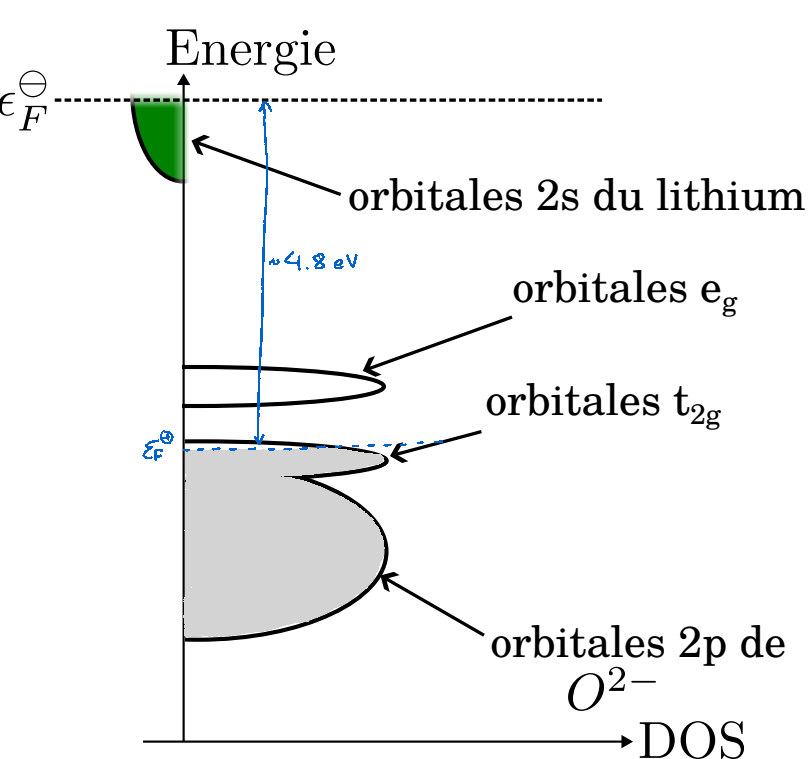
\includegraphics[width=\textwidth]{Ex18/Corr01b}
$$SoC = 100 ~ \si{\percent}$$
\end{minipage} 
\end{center}
}

On rappelle que la structure de \ce{LiCoO2} est lamellaire et que cette structure est décrite par une maille hexagonale. La structure lithiée a été suivie par DRX. On a constaté que pour $x > 0.5$, la structure ne subit aucun changement dans ses paramètres de maille. Cependant, pour $x<0.5$, on constate que le rapport $c/a$ de la maille hexagonale diminue.

\Q En vous appuyant sur la structure lamellaire, que peut traduire microscopiquement une diminution du rapport $c/a$ ?
\solution{Une diminution du rapport $c/a$ traduit le fait que l'espace entre les plaques diminue. Or, on sait que l'origine de la distance entre les plaques est électrostatique : c'est la répulsion entre les charges partielles négatives des oxygènes qui se font face.}

\Q En déduire ce qui arrive aux oxygènes.
\solution{Si la distance entre les plaques diminue, ça signifie que la répulsion entre les charges négatives est plus faible, donc tout simplement que la charge portée par l'oxygène diminue.}

\Q En vous appuyant sur le diagramme de bande, montrer que l'hypothèse \SI{100}{\percent} ionique ne permet pas de rendre compte du comportement structural observé. Que se passe-t-il ?
\solution{
On constate que lors de l'oxydation (décharge), il y a un rapprochement énergétique entre le dernier niveau occupé $t_{2g}$ du métal et le dernier niveau occupé $2p$. Or, on sait que l'interaction entre deux orbitales dépend de :
\begin{enumerate}
\item leur recouvrement ;
\item leur écart d'énergie.
\end{enumerate}
Ainsi, puisque la bande $2p$ se superpose à la bande $t_{2g}$, lors de la délithiation, ce n'est pas une orbitale $t_{2g}$ pure (modèle ionique), mais la combinaison linéaire d'une orbitale $2p-t_{2g}$ (phénomène appelé hybridation) qui soit oxydée. Ceci traduit une oxydation partielle des oxygènes.
}

\Q En vous appuyant sur une interaction selon l'axe $z$ entre une orbitale $d_{z^2}$ et une orbitale $2p_z$, montrer la différence entre l'oxydation dans un modèle purement ionique et un modèle iono-covalent.
\solution{
Dans un modèle ionique, l'écart en énergie des orbitales est suffisamment grand pour que les orbitales du métal soient les seules à perdre des électrons : 
\begin{center}
\begin{minipage}{0.48\textwidth}
\centering
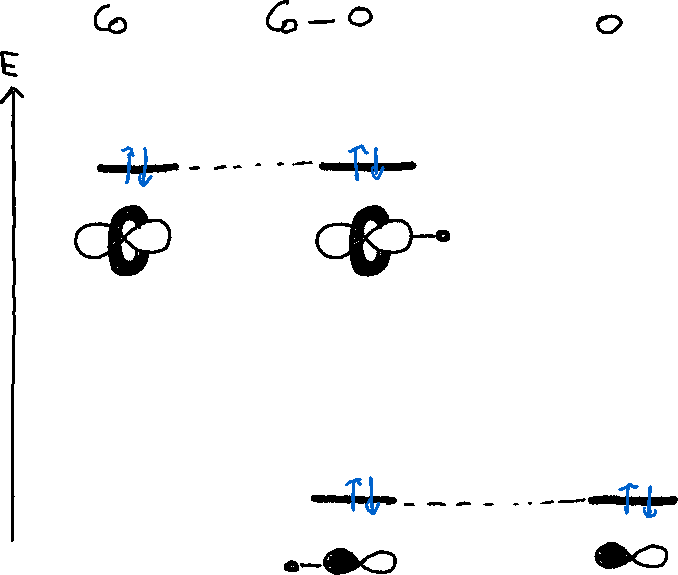
\includegraphics[width=\textwidth]{Ex18/Corr02a}
Avant oxydation
\end{minipage}\hfill \begin{minipage}{0.48\textwidth}
\centering

\includegraphics[width=\textwidth]{Ex18/Corr02b}
Après oxydation
\end{minipage}
\end{center}
Dans un modèle iono-covalent, l'orbitale oxydée présente de la densité électronique sur le métal, mais aussi, dans une moindre mesure, sur l'oxygène :
\begin{center} 
\begin{minipage}{0.48\textwidth}
\centering

\includegraphics[width=\textwidth]{Ex18/Corr02c}
Avant oxydation
\end{minipage}\hfill \begin{minipage}{0.48\textwidth}
\centering

\includegraphics[width=\textwidth]{Ex18/Corr02d}
Après oxydation
\end{minipage}\end{center}}


